\chapter{Results and interpretations}
\label{sec:results}
\section{SUSY results}
\label{sec:ssresults}

\section{SUSY interpretations}
\label{sec:ssresults}

\section{Four top results}
\label{sec:ftresults}

Distributions of the main kinematic variables (\Njets, \Nbjets, \HT, and
\ptmiss) for events in the four top analysis baseline region are shown in Fig.~\ref{fig:kinemsr} and compared
to the SM background predictions. The \Njets and \Nbjets distributions for
the CRW and CRZ are shown in Fig.~\ref{fig:kinemcr}. The expected SM \tttt
signal, normalized to its predicted cross section, is shown in both figures.
The SM predictions are statistically consistent with the observations.

\begin{figure*}[!hbt]
\centering
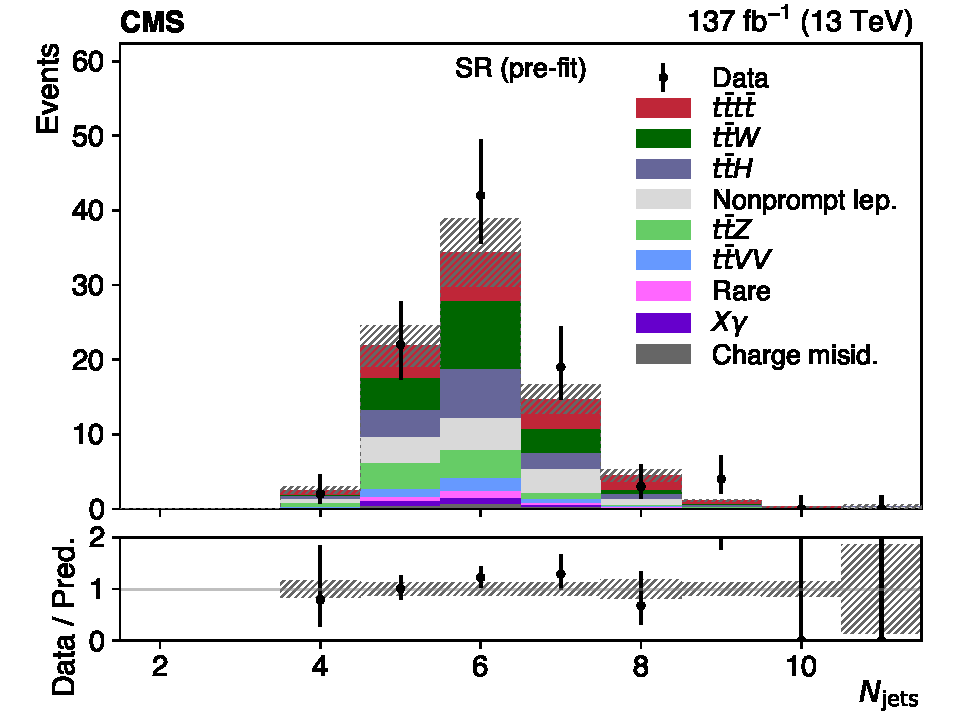
\includegraphics[width=.49\textwidth]{figs/ftp/sr_njets_prefit.pdf}
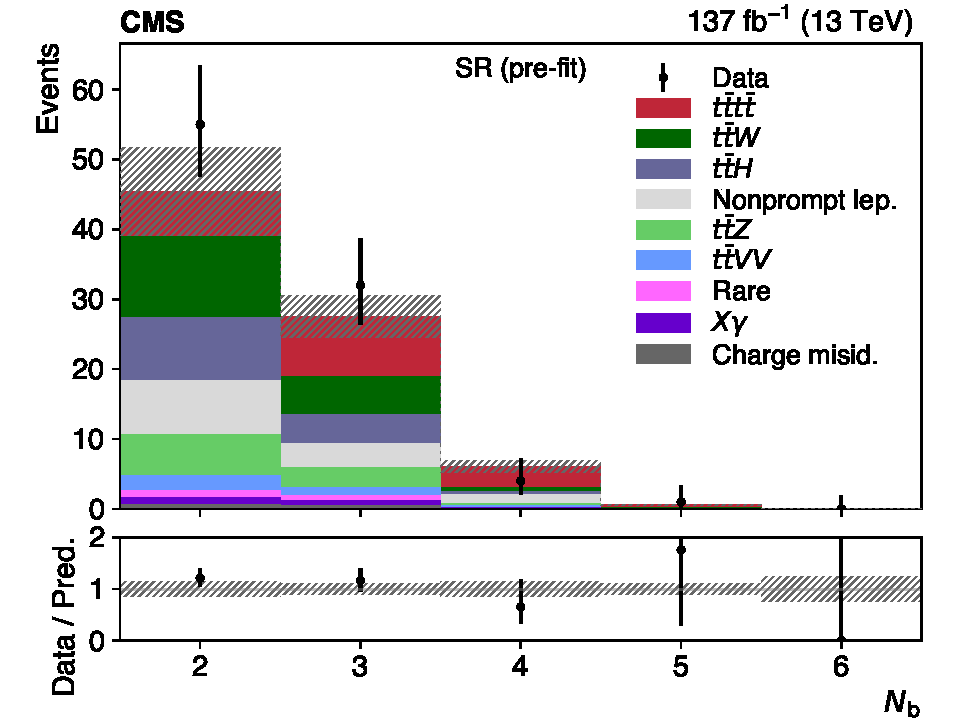
\includegraphics[width=.49\textwidth]{figs/ftp/sr_nbtags_prefit.pdf}
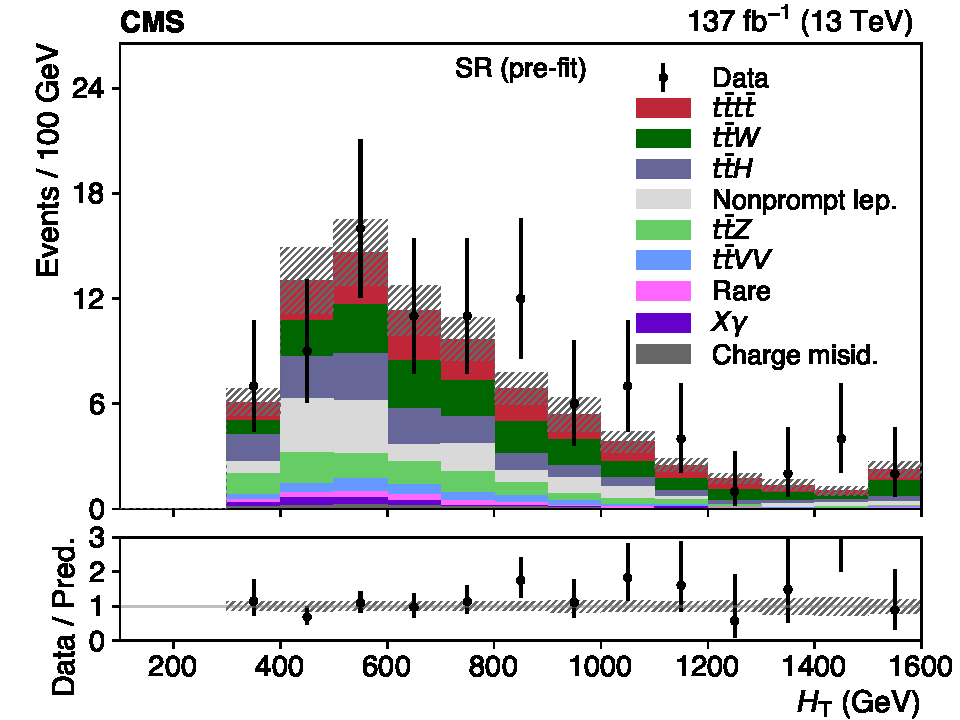
\includegraphics[width=.49\textwidth]{figs/ftp/sr_ht_prefit.pdf}
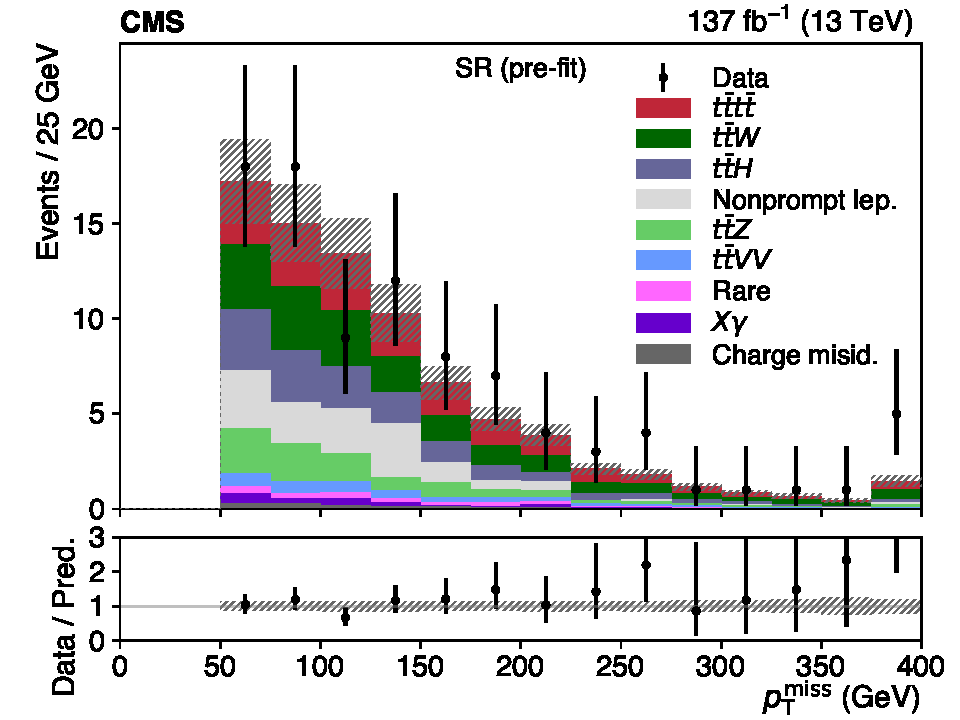
\includegraphics[width=.49\textwidth]{figs/ftp/sr_met_prefit.pdf}
\caption{ Distributions of \Njets (upper left), \Nbjets (upper right), \HT (lower left), and \ptmiss (lower right) in the summed SRs (1--14), before fitting to data,
where the last bins include the overflows. The hatched areas represent the total uncertainties in the SM signal and background predictions.
 The lower panels show the ratios of the observed event yield to the total prediction of
    signal plus background.
    }
\label{fig:kinemsr}
\end{figure*}

\begin{figure*}[!hbt]
\centering
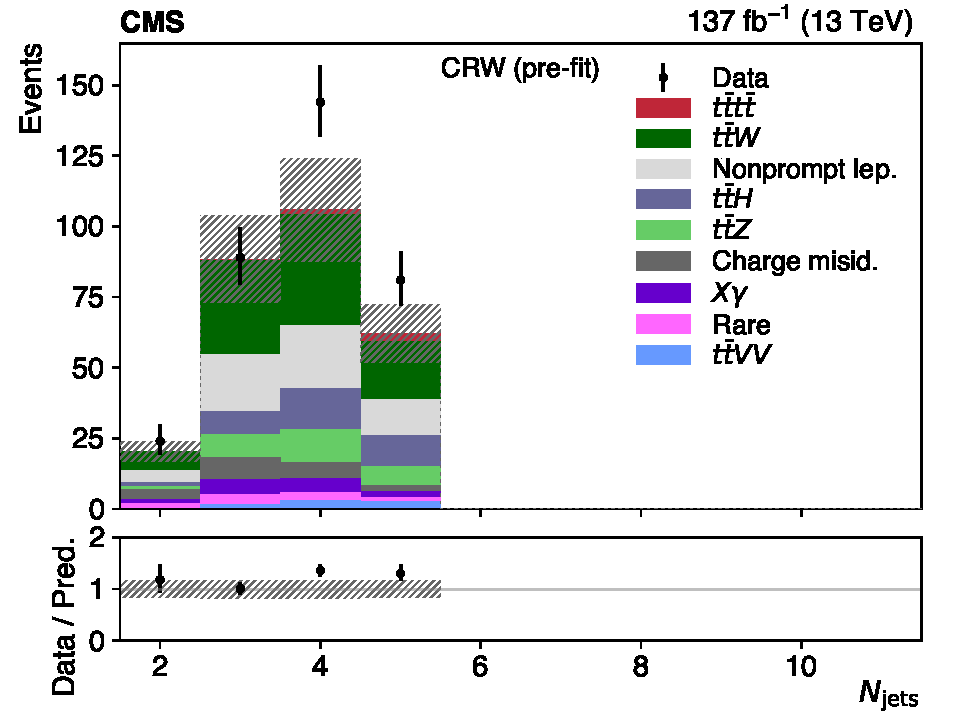
\includegraphics[width=.49\textwidth]{figs/ftp/ttwcr_njets_prefit.pdf}
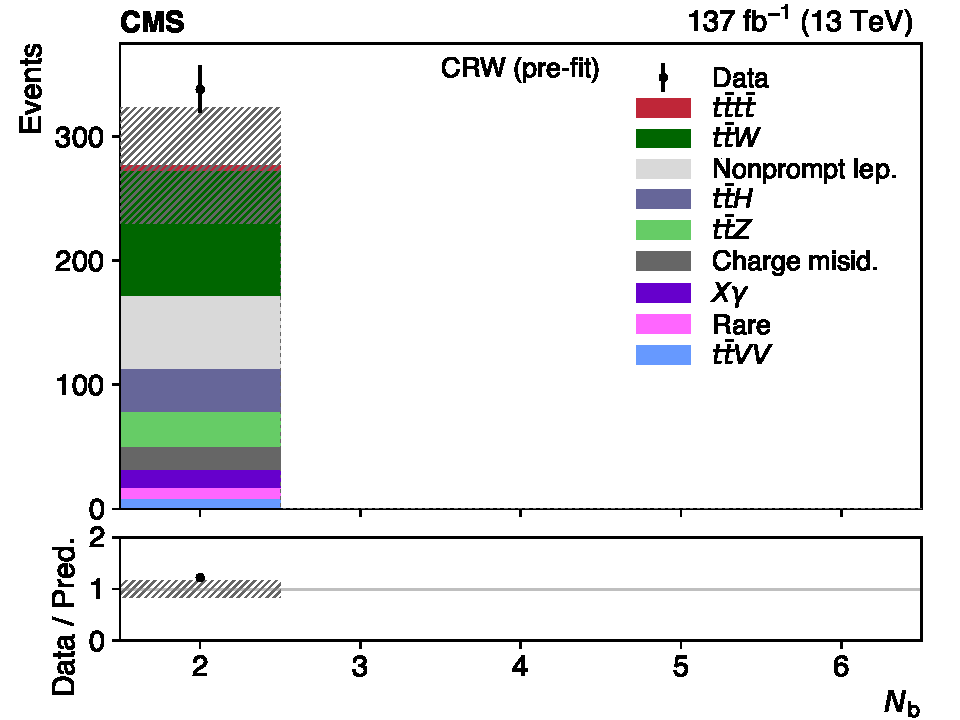
\includegraphics[width=.49\textwidth]{figs/ftp/ttwcr_nbtags_prefit.pdf}
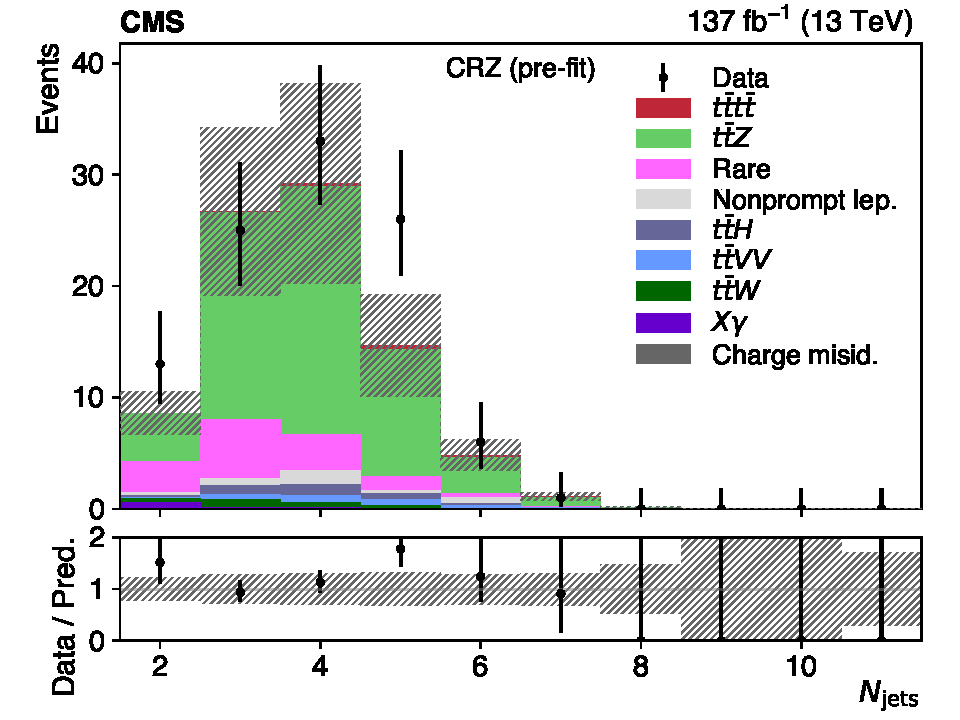
\includegraphics[width=.49\textwidth]{figs/ftp/ttzcr_njets_prefit.pdf}
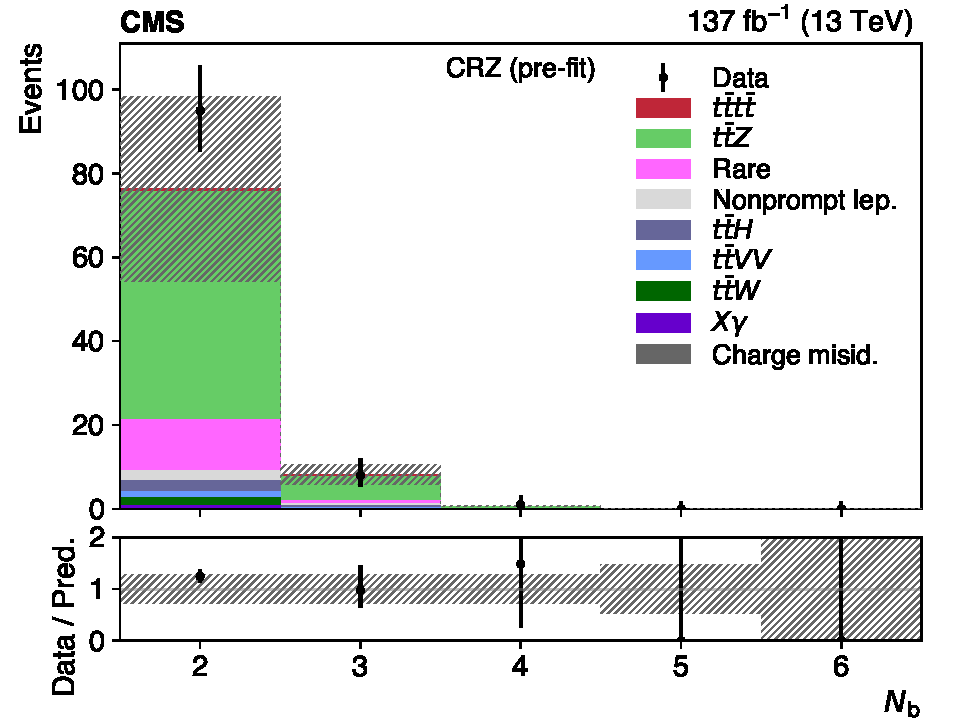
\includegraphics[width=.49\textwidth]{figs/ftp/ttzcr_nbtags_prefit.pdf}
    \caption{Distributions of \Njets (left) and \Nbjets (right) in the \ttW (upper) and \ttZ (lower) CRs, before fitting to data.
The hatched areas represent the  uncertainties in the SM signal and background predictions.
 The lower panels show the ratios of the observed event yield to the total prediction of
    signal plus background.
    }
\label{fig:kinemcr}
\end{figure*}

A binned likelihood is constructed using the yields from the signal regions,
the CRZ, as well as the CRW for the cut-based analysis only, incorporating
experimental and theoretical uncertainties as ``nuisance'' parameters. 
The measured cross
section for \tttt and the significance of the observation relative to the
background-only hypothesis are obtained from a profile maximum-likelihood
fit, in which the parameter of interest is \xsectttt and all nuisance
parameters are profiled, following the procedures described in
Refs.~\cite{STAT:ATLPHYSPUB2011011,STAT:PDG}. In addition, an upper limit at 95\%
confidence level (\CL) is set on \xsectttt using the modified frequentist
\CLs criterion~\cite{STAT:Junk1999kv,STAT:Read2002hq}, with the profile likelihood
ratio test statistic and asymptotic approximation~\cite{STAT:Cowan2010js}. We
verified the consistency between the asymptotic and fully toy-based methods.
Alternatively, by considering the SM, including the \tttt process with the SM
cross section and uncertainty~\cite{THEORY:Frederix2017wme}, as the null
hypothesis, the fit provides cross section upper limits on BSM processes with
new scalar and pseudoscalar particles.

The values and uncertainties of most nuisance parameters are unchanged by the
fit, but the ones significantly affected include those corresponding to the
\ttW and \ttZ normalizations, which are both scaled by $1.3\pm0.2$ by the
fit, in agreement with the ATLAS and CMS measurements of these
processes~\cite{ATLAS:Aaboud2019njj, CMS:Sirunyan2017uzs, CMS:2019too}. The
predicted yields after the maximum-likelihood fit (post-fit) are compared to
data in Fig.~\ref{fig:srcr} for the cut-based (upper) and BDT (lower)
analyses, where the fitted \tttt signal contribution is added to the
background predictions. The corresponding yields are shown in
Tables~\ref{tab:srcryields} and \ref{tab:srdiscyields} for the cut-based and
BDT analysis, respectively.

The \tttt cross section and the 68\% \CL interval is measured to be
$9.4^{+6.2}_{-5.6}\unit{fb}$ in the cut-based analysis, and
$12.6^{+5.8}_{-5.2}\unit{fb}$ in the BDT analysis. Relative to the
background-only hypothesis, the observed and expected significances are 1.7
and 2.5 standard deviations, respectively, for the cut-based analysis, and
2.6 and 2.7 standard deviations for the BDT analysis. The observed 95\% \CL
upper limits on the cross section are $20.0\unit{fb}$ in the cut-based and
$22.5\unit{fb}$ in the BDT analyses. The corresponding expected upper limits
on the \tttt cross section, assuming no SM \tttt contribution to the data,
are $9.4^{+4.3}_{-2.9}\unit{fb}$ (cut-based) and $8.5^{+3.9}_{-2.6}\unit{fb}$
(BDT), a significant improvement relative to the value of
$20.8^{+11.2}_{-6.9}\unit{fb}$ of Ref.~\cite{CMS:myTOP2016}. We consider the BDT
analysis as the primary result of this paper, as it provides a higher
expected measurement precision, and use the results from it for further
interpretations in the following section.




\begin{figure}[!hbtp]
\centering
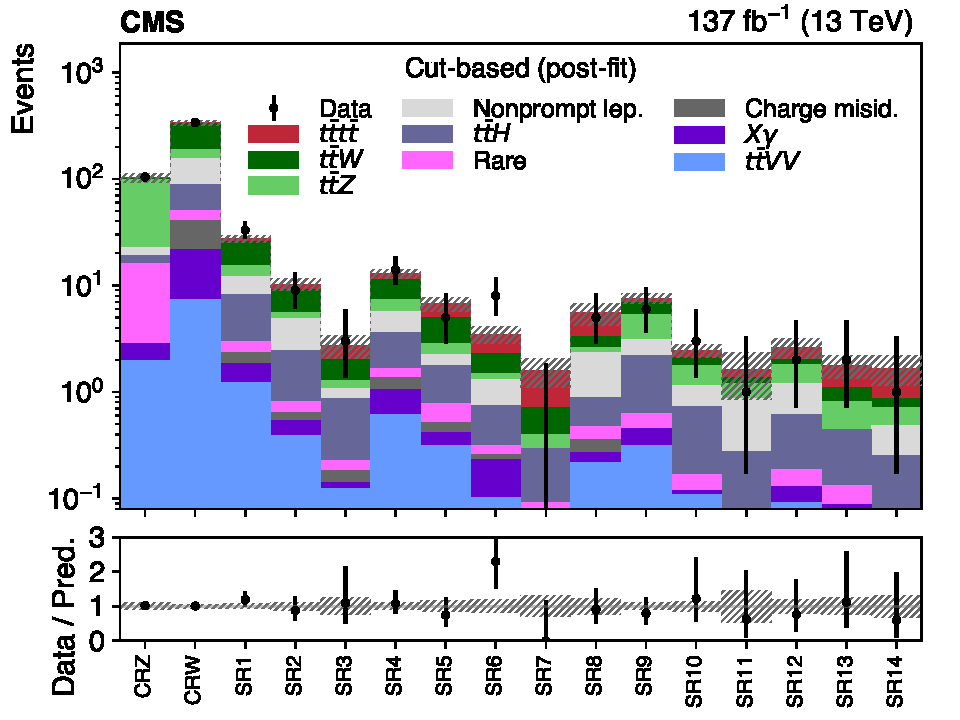
\includegraphics[width=0.8\textwidth]{figs/ftp/SRCR_postfit.pdf} \\
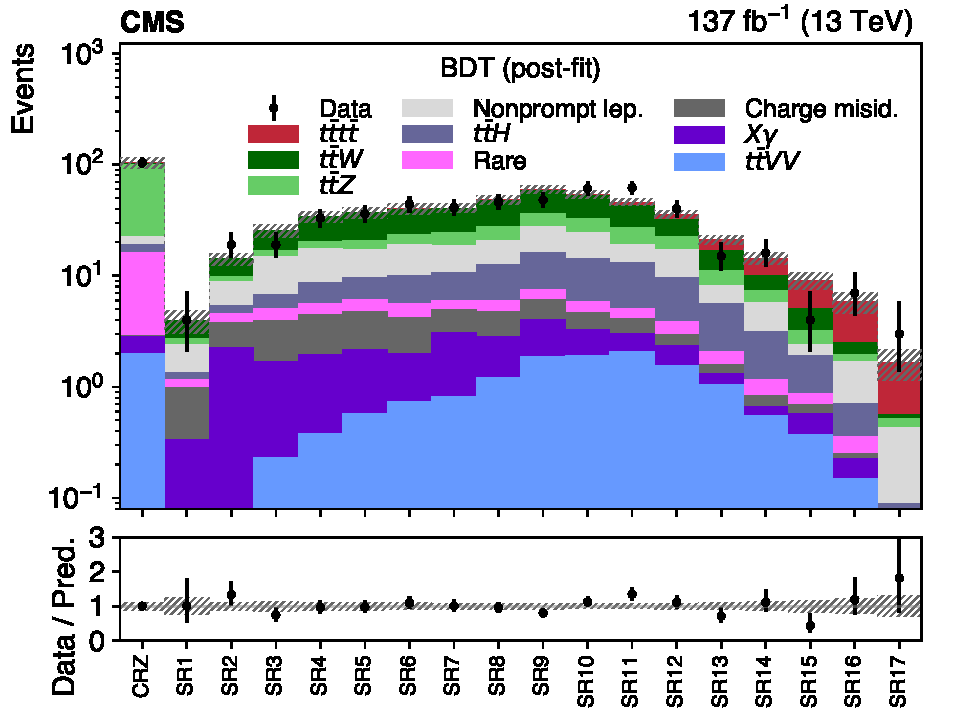
\includegraphics[width=0.8\textwidth]{figs/ftp/SRDISC_postfit.pdf}
\caption{ Observed yields in the control and signal regions for the cut-based (upper) and BDT (lower) analyses,
compared to the post-fit predictions for signal and background processes.
The hatched areas represent the total post-fit uncertainties in the signal and background predictions.
The lower panels show the ratios of the observed event yield to the total prediction of
    signal plus background.
    }
\label{fig:srcr}
\end{figure}


\begin{table*}[htb!]
\centering
    \caption{
        The post-fit predicted background, $\tttt$ signal, and total yields with
          their total uncertainties and the observed number of events
          in the control and signal regions in data for the cut-based analysis.
}
\label{tab:srcryields}
    \begin{tabular}{ccccc}
        & SM background  & $\tttt$   & Total   & Observed \\
            \hline
CRZ  & $101\pm10\ \ $   & $0.83\pm0.49$ & $102\pm10\ \ $   & 104 \\
CRW  & $331\pm19\ \ $   & $3.9\pm2.3$   & $335\pm18\ \ $   & 338 \\
SR1  & $25.6\pm2.1\ \ $ & $2.0\pm1.2$   & $27.6\pm2.1\ \ $ & 33 \\
SR2  & $9.1\pm1.3$      & $1.13\pm0.65$ & $10.3\pm1.3\ \ $ & 9 \\
SR3  & $2.01\pm0.58$    & $0.73\pm0.42$ & $2.74\pm0.67$    & 3 \\
SR4  & $11.3\pm1.3\ \ $ & $1.58\pm0.90$ & $12.9\pm1.3\ \ $ & 14 \\
SR5  & $5.03\pm0.77$    & $1.68\pm0.95$ & $6.7\pm1.1$      & 5 \\
SR6  & $2.29\pm0.40$    & $1.20\pm0.67$ & $3.48\pm0.66$    & 8 \\
SR7  & $0.71\pm0.20$    & $0.88\pm0.48$ & $1.59\pm0.49$    & 0 \\
SR8  & $3.31\pm0.95$    & $2.2\pm1.3$   & $5.5\pm1.3$      & 5 \\
SR9  & $6.84\pm0.80$    & $0.71\pm0.39$ & $7.55\pm0.80$    & 6 \\
SR10 & $2.10\pm0.31$    & $0.35\pm0.22$ & $2.45\pm0.35$    & 3 \\
SR11 & $1.38\pm0.75$    & $0.23\pm0.14$ & $1.61\pm0.75$    & 1 \\
SR12 & $2.03\pm0.48$    & $0.59\pm0.34$ & $2.62\pm0.54$    & 2 \\
SR13 & $1.09\pm0.28$    & $0.69\pm0.39$ & $1.78\pm0.44$    & 2 \\
SR14 & $0.87\pm0.30$    & $0.80\pm0.45$ & $1.67\pm0.52$    & 1 \\
\end{tabular}
\end{table*}




\begin{table*}[htb!]
\centering
    \caption{
        The post-fit predicted background and $\tttt$ signal, and total yields with
          their total uncertainties and the observed number of events
          in the control and signal regions in data for the BDT analysis.
}
\label{tab:srdiscyields}
    \begin{tabular}{ccccc}
        & SM background  & $\tttt$   & Total   & Observed \\
            \hline

CRZ  & $102\pm12\ \ $   & $1.11\pm0.43$ & $103\pm12\ \ $   & 104 \\
SR1  & $3.95\pm0.96$    & $ <0.01 $     & $3.96\pm0.96$    & 4 \\
SR2  & $14.2\pm1.8\ \ $ & $0.01\pm0.01$ & $14.2\pm1.8\ \ $ & 19 \\
SR3  & $25.5\pm3.5\ \ $ & $0.04\pm0.03$ & $25.6\pm3.5\ \ $ & 19 \\
SR4  & $34.0\pm4.0\ \ $ & $0.08\pm0.05$ & $34.0\pm4.0\ \ $ & 33 \\
SR5  & $36.7\pm4.0\ \ $ & $0.15\pm0.07$ & $36.8\pm4.0\ \ $ & 36 \\
SR6  & $39.8\pm4.2\ \ $ & $0.23\pm0.12$ & $40.0\pm4.2\ \ $ & 44 \\
SR7  & $40.3\pm3.7\ \ $ & $0.31\pm0.16$ & $40.6\pm3.8\ \ $ & 41 \\
SR8  & $47.3\pm4.3\ \ $ & $0.72\pm0.28$ & $48.0\pm4.3\ \ $ & 46 \\
SR9  & $58.5\pm5.2\ \ $ & $1.18\pm0.46$ & $59.7\pm5.2\ \ $ & 48 \\
SR10 & $52.1\pm4.3\ \ $ & $1.91\pm0.74$ & $54.1\pm4.2\ \ $ & 61 \\
SR11 & $43.0\pm3.5\ \ $ & $3.0\pm1.2$   & $46.0\pm3.5\ \ $ & 62 \\
SR12 & $32.1\pm3.0\ \ $ & $3.7\pm1.4$   & $35.8\pm2.9\ \ $ & 40 \\
SR13 & $16.7\pm1.6\ \ $ & $4.3\pm1.6$   & $21.0\pm2.0\ \ $ & 15 \\
SR14 & $10.1\pm1.2\ \ $ & $4.2\pm1.6$   & $14.3\pm1.8\ \ $ & 16 \\
SR15 & $5.03\pm0.77$    & $4.1\pm1.5$   & $9.1\pm1.6$      & 4 \\
SR16 & $2.49\pm0.61$    & $3.4\pm1.3$   & $5.9\pm1.3$      & 7 \\
SR17 & $0.57\pm0.36$    & $1.08\pm0.42$ & $1.65\pm0.50$    & 3 \\

\end{tabular}

\end{table*}

\section{Four top interpretations}
\label{sec:ftinterpretations}

This analysis is used to constrain SM parameters, as well as production of
BSM particles and operators that can affect the \tttt production rate. The
existence of \tttt Feynman diagrams with virtual Higgs bosons allows
interpreting the upper limit on \xsectttt as a constraint on the Yukawa
coupling, $y_{\PQt}$, between the top quark and the Higgs
boson~\cite{THEORY:TopYukawaTTTT, THEORY:TopYukawaTTTTnew}. Similarly, the
measurement can be interpreted as a constraint on the Higgs boson oblique
parameter $\hat{H}$, defined as the Wilson coefficient of the dimension-six
BSM operator modifying the Higgs boson propagator~\cite{THEORY:ObliqueHiggs2019}.
More generically, Feynman diagrams where the virtual Higgs boson is replaced
by a virtual BSM scalar ($\phi$) or vector ($\cPZpr$) particle with mass
smaller than twice the top quark mass ($m < 2m_\PQt$), are used to interpret
the result as a constraint on the couplings of such new
particles~\cite{THEORY:Alvarez2016nrz}. In addition, new particles with $m >
2m_\PQt$, such as a heavy scalar (\PH) or pseudoscalar (\PSA), can be
produced on-shell in association with top quarks. They can subsequently decay
into top quark pairs, generating final states with three or four top quarks.
Constraints on the production of such heavy particles can be interpreted in
terms of 2HDM parameters~\cite{THEORY:Dicus1994bm,THEORY:Craig2015jba,THEORY:Craig2016ygr},
or in the framework of simplified models of dark matter~\cite{THEORY:Boveia2016mrp,
THEORY:Albert2017onk}.

When using our \tttt to determine a constraint on $y_{\PQt}$, we verified
using a LO simulation that the signal acceptance is not affected by the
relative contribution of the virtual Higgs boson Feynman diagrams. We take
into account the dependence of the backgrounds on $y_{\PQt}$ by scaling the
\ttH cross section by $\abs{y_{\PQt}/y_{\PQt}^{\mathrm{SM}}}^2$ prior to the
fit, where $y_{\PQt}^{\mathrm{SM}}$ represents the SM value of the top quark
Yukawa coupling. As a result of the \ttH background rescaling, the measured
\xsectttt depends on $\abs{y_{\PQt}/y_{\PQt}^{\mathrm{SM}}}$, as shown in
Fig.~\ref{fig:yukawa}. The measurement is compared to the theoretical
prediction obtained from the LO calculation of Ref.~\cite{THEORY:TopYukawaTTTT},
scaled to the $12.0^{+2.2}_{-2.5}\unit{fb}$ cross section obtained in
Ref.~\cite{THEORY:Frederix2017wme}, and including the uncertainty associated with
doubling and halving the renormalization and factorization scales. Comparing
the observed limit on \xsectttt with the central, upper, and lower values of
its theoretical prediction, we obtain 95\% \CL limits of
$\abs{y_{\PQt}/y_{\PQt}^{\mathrm{SM}}} < 1.7$, $1.4$, and $2.0$,
respectively, an improvement over the previous CMS
result~\cite{CMS:myTOP2016}. Alternatively, assuming that the on-shell Yukawa
coupling is equal to that of the SM, we do not rescale the \ttH background
with respect to its SM prediction, and obtain corresponding limits on the
off-shell Yukawa coupling of $\abs{y_{\PQt}/y_{\PQt}^{\mathrm{SM}}} < 1.8$,
$1.5$, and $2.1$. Since $y_{\PQt}$ affects the Higgs boson production cross
section in both the gluon fusion and \ttH modes, constraints on $y_{\PQt}$
can also be obtained from a combination of Higgs boson
measurements~\cite{STAT:AtlasCmsHiggsComb}. However, these constraints require
assumptions about the total width of the Higgs boson, while the \tttt-based
limit does not. For the $\hat{H}$ interpretation, the BDT analysis is
repeated using simulated samples of \tttt signal events with different values
of $\hat{H}$ to account for small acceptance and kinematic differences. 
We rescale the \ttH cross section by
$(1-\hat{H})^2$ to account for its $\hat{H}$
dependency~\cite{THEORY:ObliqueHiggs2019}. This results in the 95\% \CL upper limit
of $\hat{H} < 0.12$. For reference, the authors of
Ref.~\cite{THEORY:ObliqueHiggs2019} used recent LHC on-shell Higgs boson
measurements to set a constraint of $\hat{H} < 0.16$ at 95\% \CL.


To study the off-shell effect of new particles with $m < 2m_\PQt$, we first
consider neutral scalar ($\phi$) and neutral vector ($\cPZpr$) particles that
couple to top quarks. Such particles are at present only weakly constrained,
while they can give significant contributions to the \tttt cross
section~\cite{THEORY:Alvarez2016nrz}. Having verified in LO simulation that these
new particles affect the signal acceptance by less than 10\%, we recalculate
the \xsectttt upper limit of the BDT analysis including an additional 10\%
uncertainty in the acceptance, and obtain the 95\% \CL upper limit of
23.0\unit{fb} on the total \tttt cross section, slightly weaker than the
22.5\unit{fb} limit obtained in Section~\ref{sec:results}. Comparing this
upper limit to the predicted cross section in models where \tttt production
includes a $\phi$ or a $\cPZpr$ in addition to SM contributions and
associated interference, we set limits on the masses and couplings of these
new particles, shown in Fig.~\ref{fig:ZprimePhiExclusions}. These limits
exclude couplings larger than 1.2 for $m_{\phi}$ in the 25--340\GeV range and
larger than 0.1 (0.9) for $m_{\cPZpr} = 25$ (300)\GeV.

We consider on-shell effects from new scalar and pseudoscalar particles with $m > 2m_\PQt$. At such masses, the production rate of these particles
in association with a single top quark ($\PQt\PQq\PH/\PSA$, $\PQt\PW\PH/\PSA$) becomes significant,
so we include these processes in addition to $\PQt\overline{\PQt}\PH/\PSA$.
As pointed out in Ref.~\cite{THEORY:Craig2016ygr}, these processes do not suffer significant interference with the SM \tttt process.
To obtain upper limits on the sum of these processes followed by the decay $\PH/\PSA\to \ttbar$,
we use the BDT analysis and treat the SM \tttt process as a background.
Figure~\ref{fig:HiggsLimits} shows the excluded cross section as a function of the mass of the scalar (left) and pseudoscalar (right).
Comparing these limits with the Type-II 2HDM cross sections with $\tan\beta = 1$ in the alignment limit,
we exclude scalar (pseudoscalar) masses up to 470~(550)\GeV, improving by more than 100\GeV with respect to the previous CMS limits~\cite{CMS:mySUS2016}.
Alternatively, we consider the simplified model of dark matter defined in Ref.~\cite{CMS:DMsingletop},
which includes a Dirac fermion dark matter candidate, $\chi$, in addition to $\PH/\PSA$, and where the couplings of $\PH/\PSA$
to SM fermions and $\chi$ are determined by parameters $g_\mathrm{SM}$ and $g_\mathrm{DM}$, respectively.
In this model, exclusions similar to those from 2HDM are reached by assuming $g_\mathrm{SM} = 1$ and $g_\mathrm{DM} = 1$,
and taking  $m_{\PH/\PSA} < 2 m_\chi$.
Relaxing the 2HDM assumption of $\tan\beta = 1$, Fig.~\ref{fig:HiggsLimitsTB} shows the 2HDM limit as a function of $\PH/\PSA$ mass and $\tan\beta$,
considering one new particle at a time and also including a scenario with  $m_\PH = m_\PSA$ inspired by
a special case of Type-II 2HDM, the hMSSM~\cite{THEORY:Djouadi2013uqa}.
Values of $\tan\beta$ up to 0.8--1.6 are excluded, depending on the assumptions made.
These exclusions are comparable to those of a recent CMS search for the resonant production of $\PH/\PSA$ in the
$\Pp\to \PH/\PSA \to \ttbar$ channel~\cite{CMS:HIG17027}.
Relaxing the $m_{\PH/\PSA} < 2 m_\chi$ assumption in the dark matter model, Fig.~\ref{fig:DMLimits} shows the
limit in this model as a function of the masses of both $\PH/\PSA$ and $\chi$,
for $g_\mathrm{DM} = 1$ and for two different assumptions of $g_\mathrm{SM}$.
Large sections of the phase space of simplified dark matter models are excluded, and the reach of this analysis is complementary
to that of analyses
considering decays of $\PH/\PSA$ into invisible dark matter candidates, such as those of Refs.~\cite{CMS:DMsingletop, ATLAS:Aaboud2017rzf}.

\begin{figure}[!hbtp]
\centering
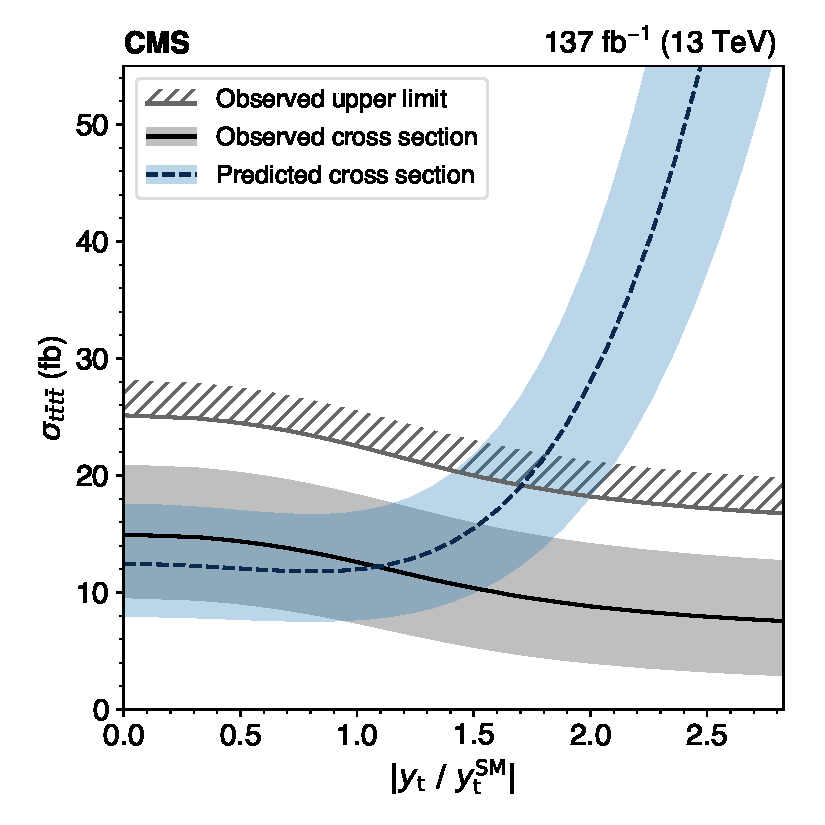
\includegraphics[width=.49\textwidth]{figs/ftp/yukawa.pdf}
\\
\caption{
    The observed \xsectttt (solid line) and 95\% \CL upper limit (hatched line) are shown as a function
    of $\abs{y_{\PQt}/y_{\PQt}^{\mathrm{SM}}}$. The predicted value (dashed line)~\cite{THEORY:TopYukawaTTTT},
    calculated at LO and scaled to the calculation from Ref.~\cite{THEORY:Frederix2017wme}, is also plotted.
    The shaded band around the measured value gives the total uncertainty, while the shaded band around
    the predicted curve shows the theoretical uncertainty associated with the renormalization and
    factorization scales.
}
\label{fig:yukawa}
\end{figure}

\begin{figure}[!hbtp]
\centering
    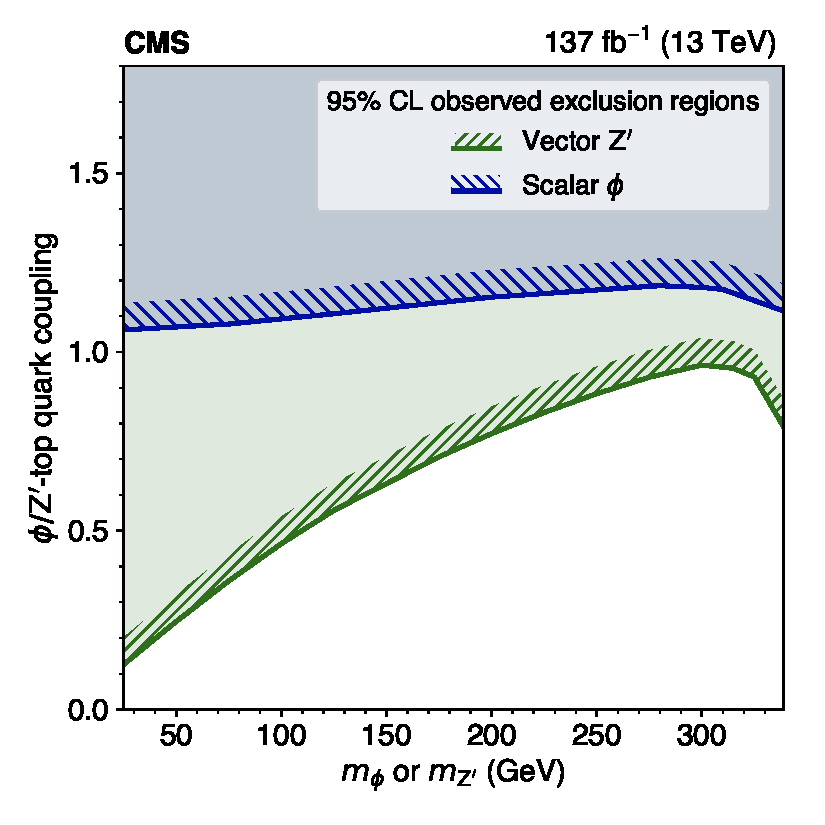
\includegraphics[width=.49\textwidth]{figs/ftp/plot_2d_phizprime.pdf}
\caption{
    The 95\% \CL exclusion regions in the plane of the $\phi/\cPZpr$-top quark coupling versus
    $m_{\phi}$ or $m_{\cPZpr}$. The excluded regions are above the hatched lines.
    }
\label{fig:ZprimePhiExclusions}
\end{figure}

\begin{figure*}[!hbtp]
\centering
    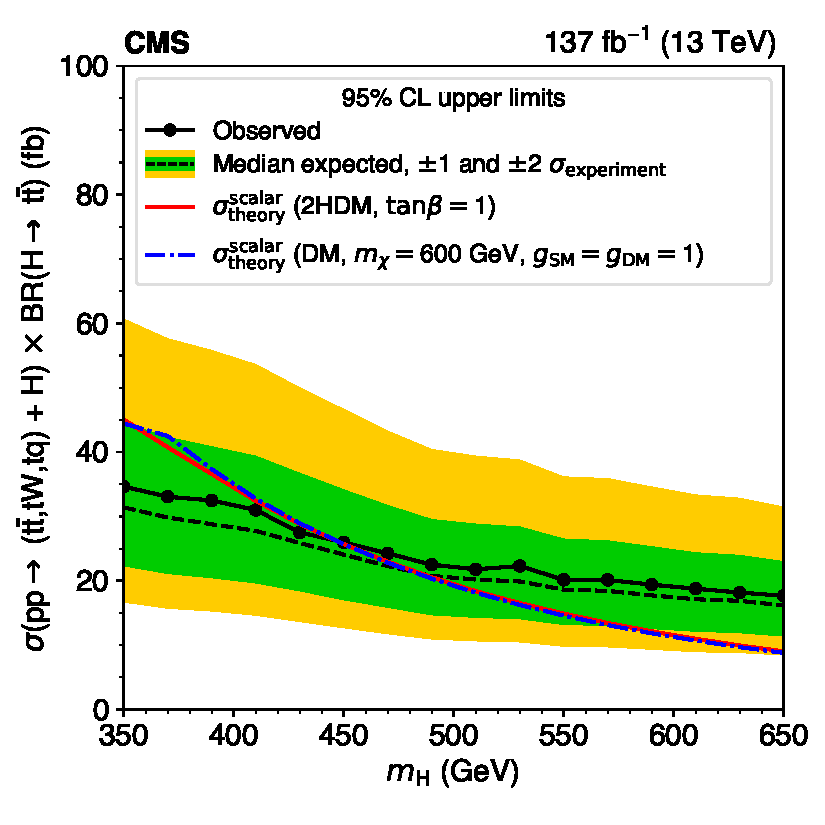
\includegraphics[width=.49\textwidth]{figs/ftp/ft_higgs_sc_scan_limit.pdf}
    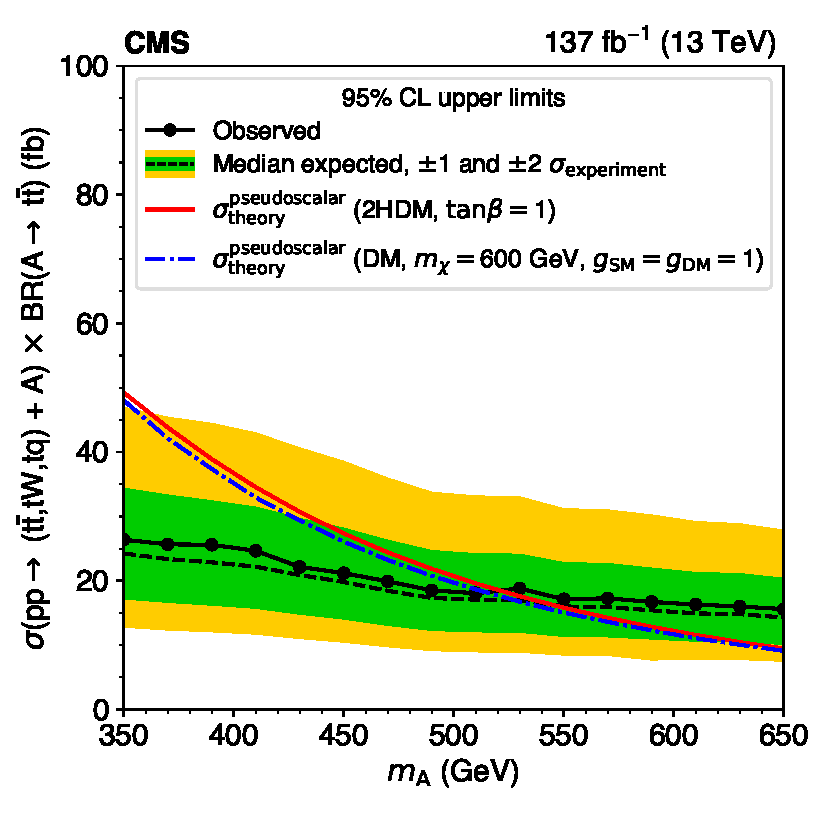
\includegraphics[width=.49\textwidth]{figs/ftp/ft_higgs_ps_scan_limit.pdf}
\caption{
    The observed (points) and expected (dashed line) 95\% \CL upper limits on the cross section
    times branching fraction to \ttbar for the production of a new heavy scalar \PH (left) and pseudoscalar \PSA (right),
    as a function of mass. The inner and outer bands around the expected limits indicate the regions containing 68 and 95\%,
    respectively, of the distribution of limits under the background-only hypothesis. Theoretical values are shown for Type-II 2HDM
    in the alignment limit (solid line) and simplified dark matter (dot-dashed line) models.
}
\label{fig:HiggsLimits}
\end{figure*}

\begin{figure*}[!hbtp]
\centering
    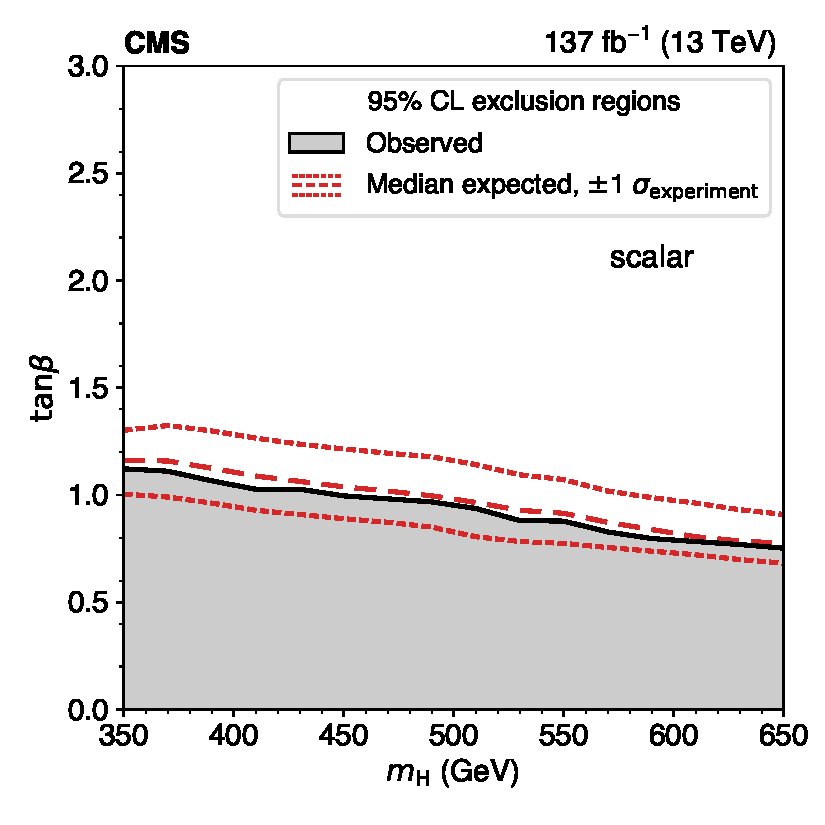
\includegraphics[width=.49\textwidth]{figs/ftp/plot_2d_2hdm_tanbetaexclusion_h.pdf}
    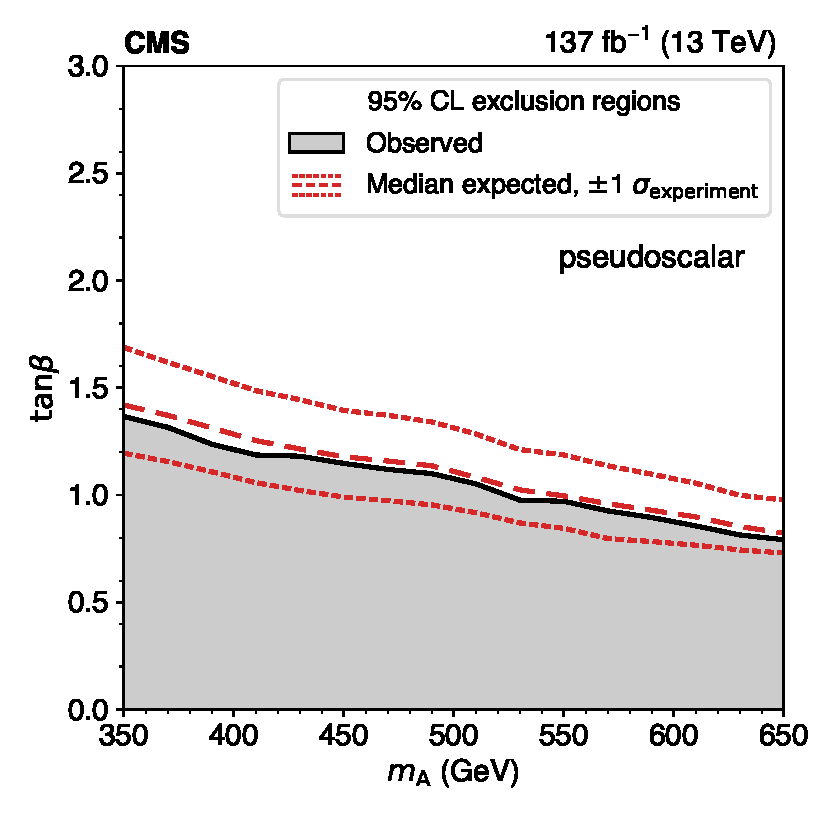
\includegraphics[width=.49\textwidth]{figs/ftp/plot_2d_2hdm_tanbetaexclusion_a.pdf}
    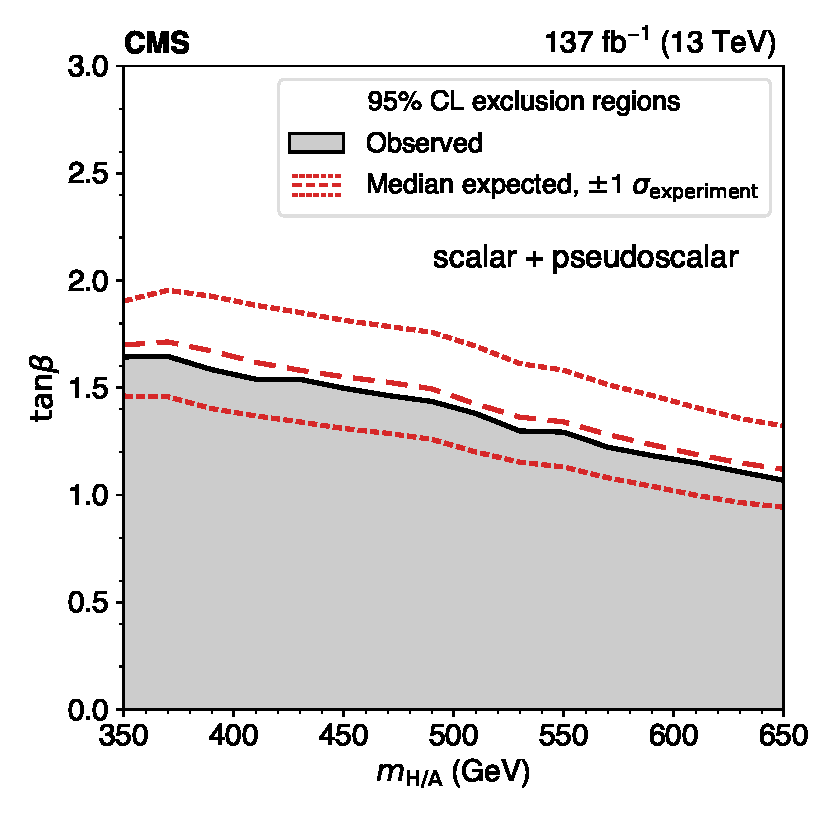
\includegraphics[width=.49\textwidth]{figs/ftp/plot_2d_2hdm_tanbetaexclusion_b.pdf}
\caption{
    The observed (solid curve) and expected (long-dashed curve) 95\% \CL exclusion regions in the $\tan\beta$ versus mass plane
    for Type-II 2HDM models in the alignment limit for a new scalar \PH (upper left), pseudoscalar \PSA (upper right), and both (lower) particles.
    The short-dashed curves around the expected limits indicate the region containing 68\% of the distribution of limits expected under the
    background-only hypothesis. The excluded regions are below the curves.
}
\label{fig:HiggsLimitsTB}
\end{figure*}

\begin{figure*}[!hbtp]
\centering
    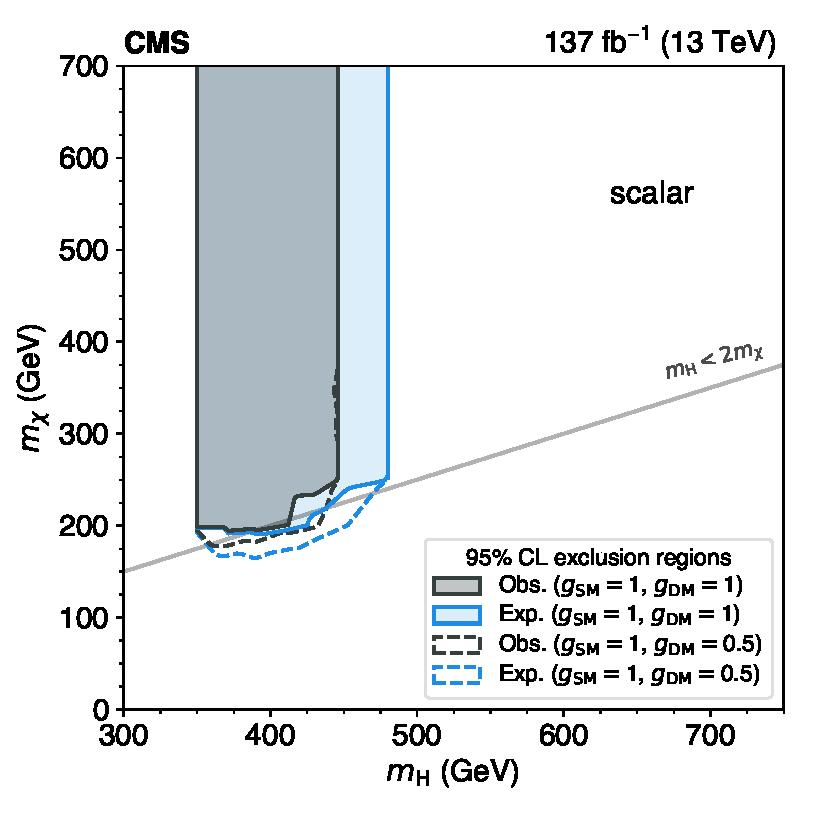
\includegraphics[width=.49\textwidth]{figs/ftp/plot_2d_dmscalar_xsec_totsm_bothcouplings.pdf}
    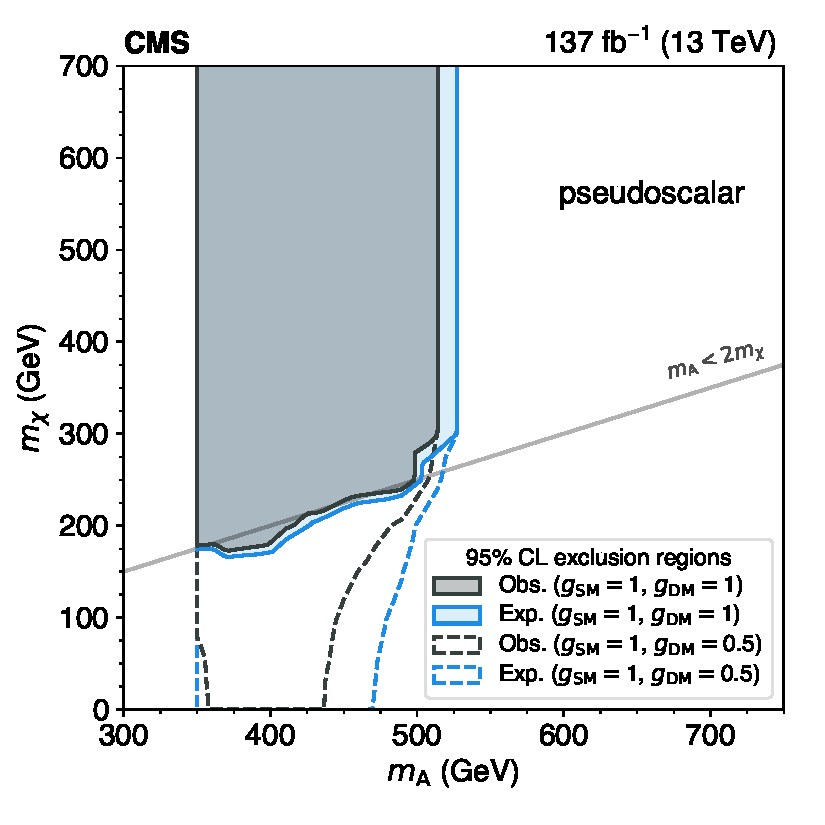
\includegraphics[width=.49\textwidth]{figs/ftp/plot_2d_dmpseudo_xsec_totsm_bothcouplings.pdf}
\caption{
	Exclusion regions at 95\% \CL in the plane of $m_\chi$ vs. $m_{\PH}$ (left) or $m_{\PSA}$ (right).
    The outer lighter and inner darker solid curves show the expected and observed limits, respectively,
    assuming $g_\mathrm{SM} = g_\mathrm{DM} = 1$. The excluded regions, shaded, are above the limit curves.
    The dashed lines show the limits assuming a weaker coupling between $\PH/\PSA$ and $\chi$, $g_\mathrm{DM} = 0.5$.
    }
\label{fig:DMLimits}
\end{figure*}
